\section{Background}

In this section a comparison of physics world simulators and state of the art exoskeletons that attempt to incorporate touch into virtual environments will be made.

\subsection{Virtual environment}
The hard requirements
for the choice of the simulator for this thesis are simple, it must have:
\begin{enumerate}
  \item VR support. Users should be able to interact with the environment.
  \item Support of the soft-body physics.
\end{enumerate}
\noindent
A great to have features for the simulator are the following:
\begin{enumerate}
  \item Free and open-source, so the research in this thesis could be easily accesible and replicated.
  \item Fast, so the development would go smoothly on an affordable computer.
  \item Popular, it is easier to fix problems if we can find people in forums who already had them.
  \item Easy to learn, it would be great to have more time on research and implementation than learning the engine.
  \item Used in robotics applications.
\end{enumerate}
Numerous physics engines have been developed in which virtual environemnts can be created. Most notable are \cite{physics_simulators_review}: Mujoco, Gazebo, CoppeliaSim, Webots, PyBullet and SOFA.

\bigskip \noindent
Multi-Joint dynamics with Contact (MuJoCo) \cite{mujoco} is a popular physics engine that required
a commercial license up until recently. In 2021 Google Deepmind acquired the simulator and made it
freely available for everyone \cite{deepmind2021mujoco}. In 2022, they open-sourced and published it on Github. The MuJoCo is widely used in research due to its contact stability \cite{app13020680}. State of the art research leverages MuJoCo for training robotic manipulator policies in simulation. It is worth noting that MuJoCo lacks built-in functionality for inverse kinematics or path planning.

\bigskip \noindent
Gazebo is another popular robotics simulator that is widely used in research. One of the things that makes it so appealing is support of Robotics Operating System \cite{ros} (ROS). ROS houses a expansive set of libraries and tools
for building robotics applications. ROS-based software is platform and language agnostic making incorporation of user developed libraries very easy. The working principle that allows for this seamless integration is Publish/Subscribe model. ROS processes called nodes, communicate between each other by publishing
messages to topics and receiving messages from subscribed
topics allowing interprocess communication. A study has shown that if the robot model in Gazebo was created properly, the code that was used in simulation can be directly reused in real robot without any modifications \cite{ros-gazebo-integration}. Unfortnately the engine does not support soft-body physics natively. There are however attempts to bridge this gap between rigid-body and soft-body physics. One study developed a ROS-Gazebo Toolbox that allows user to bring Articulated Soft Robots in the simulation with satisfactory Sim2Real performance \cite{Mengacci2021}

\bigskip \noindent
CoppeliaSim, formerly known as V-REP \cite{coppelia}, has an easy learning curve with it's GUI driven design and user-
centric feature including forward and inverse kinematics, sensor simulation, motion and path planning. Built around a distributed control architecture, the engine supports scripts written in Lua or Python and plugins written in C/C++ that act as synchronous controllers. This is useful in multi-robot setups. It also has ROS support, but unlike Gazebo, it is secondary to the engine's design. CoppeliaSim supports 5 different physics engines (MuJoCo, Bullet Physics, ODE, Newton and Vortex Dynamics), but the support for soft body and deformable objects is lacking.

\bigskip \noindent
Webots \cite{michel2004cyberbotics}, started in 1996, is an open-source simulator witten in C++. It has a large collection of sensors, actuator and robot models. The simulator is beginner friendly with polished GUI that makes it easy to build models from scratch. One study comparing robot simulators has shown that Webots was least resource intensive, it the lowest CPU usage compared to CoppeliaSim and Gazebo \cite{DBLP:journals/corr/abs-2008-04627}. These reasons make the simulator appealing for fast prototyping and multi-robot simulation purposes. Despite these great features the simulator lacks soft-body dynamics support.

\bigskip \noindent
Bullet is a professional library written in C++. It is videly used in games, visual effects and robotics applications. It can simulate Soft-Body as well as Rigid-Body physics with discrete and continuous collision detection. The PyBullet is a library with Python bindings that interact with the Bullet engine. This approach merges best of both worlds, the C++ speed and Python's ease of use. PyBullet also has reinforcement learning, robotics simulation and VR support. 

\begin{table}[tb] % placement: h for here, t for top, b for bottom
  \centering
  \begin{tabular}{l c c c c c}  % two columns: l for left, c for center, r for right
    Simulator & Force Sensor & Inverse Kinematics & Soft-Body & VR & ROS
 \\\hline
 MuJoCo & \cmark & \xmark & \cmark & \cmark & \xmark
 \\
 Gazebo & \cmark & \cmark & \xmark & \cmark & \cmark
 \\
 CoppeliaSim & \cmark & \cmark & \xmark & \cmark & \cmark
 \\
 Webots & \cmark & \xmark & \xmark & \cmark & \cmark
 \\
 PyBullet & \cmark & \cmark & \cmark & \cmark & \xmark
  \end{tabular}
  \caption{Feature Comparison of Popular Physics Simulators for Robotics Applications}
  \label{tab:robot-advantages}
\end{table}

\bigskip \noindent
From the examined physics engines only MuJoCo and PyBullet support deformable objects and virtual reality. PyBullet was chosen as the physics engine for this thesis as it has a well documented VR section and broader VR support. Teleoperation with MuJuCo is only avaialble through the use of MuJoCo HAPTIX \cite{7363441} whereas PyBullet support a variety of VR controllers.

\subsection{Exoskeletons}
The human skin is the largest organ of the body, it plays a crucial role in the perception of touch and temperature. The density of touch receptors varies significantly across different skin regions. The palms of the hand, especially fingertips are one of the most touch sensitive parts of the body. These areas have a heightened sensitivity, because hands serve as the primary interface for interacting with the environment, feeling the objects temperature, texture and weight. Given the complexity and cost associated with the development of a full body exoskeleton, the focus of this thesis will exclusively be on create an exoskeleton for the hand only. There have already been multiple attempts to create an exoskeleton that enable user to feel the virtual objects. Some of which have even became commercially available.

\subsubsection{Types of Feedback}
There are multiple forms of haptic feedback a simple touch can provide. This section explore the different types of feedback and their significance in virtual interactions.

\bigskip \noindent
Transient contact and normal force play a fundamental role in perceiving the stiffness of an object. One study has shown that transient vibration combined with visuo-haptic illusion could successfully simulate this form of contact \cite{9117062}. The results indicate that this type of contact can be modeled without requiring complex mechatronic or control systems.

\bigskip \noindent
Lateral stretch of the skin provide information about the weight of the object, while the stick-slip condition offers insight into when an object is about to be dropped. This information allows people to instinctively react by either gripping the object tighter to prevent slippage or try to catch it mid-air if it has already slipped. Various approaches and design methodologies have been investigated to replicate these tactile sensations in virtual environments \cite{10.1145/1278280.1278289}\cite{10.1145/3126594.3126599}.

\bigskip \noindent
Beyond force, pressure and friction feedback, the human skin is also adept at recognizing the texture of the objects. One study has shown that it is feasible to simulate texture perception using vibratory-only
feedback by leveraging the spatial information of skin interactions with textured surfaces \cite{article2615616}. This suggests that a combination of finely tuned vibrations and high-resolution sensor data could enable realistic textural perception in virtual environments.

\bigskip \noindent
Temperature feedback is another important component of realistic haptic interactions. Temperature can provide important information about the type of material we are in contact with. Different heat flows and temperature gradients are experienced when touching objects due to the different thermal conductivity coefficients between materials. For example, when touching a metal or a wooden surface, even if both objects are at the same temperature, the metal will feel significantly colder than the wood. This is because the metal has much greater thermal conductivity than the wood. A wearable device that achieves temperature feedback has been proposed for the VR setting \cite{10.1007/978-3-030-58147-3_32}. It contains a film with high thermal conductivity controller by Peltier element, which is coupled with a water-cooling heatsink in order to achieve the dynamic temperature simulation.

\bigskip \noindent
Although various studies have proposed solutions that simulate the individual aspects of the sense of touch, integrating multiple feedback modalities into a single, compact and lightweight exoskeleton remains a formidable engineering challenge. Combining force, texture, temperature, and friction feedback into a light, ergonomic and mass produced glove could be the goal for the future of haptic systems, however this thesis will exclusively focus on incorporating the sense the normal force exerted by the objects, as this is arguably the most important aspect of the touch as it allows users to feel the presence of the object.

\subsubsection{Tracking}
Hand tracking can be divided into two main categories: global position tracking and local position tracking. Global position tracking determines the whereabouts of the hand's location in the world space and local position tracking provides detailed information on the configuration and movement of the hand.
Several technologies exist that can be attached to the exoskeleton to provide global position tracking.

\bigskip \noindent
Vive Tracker, the first commercially available VR tracker developed by HTC enable object and body tracking in virtual reality environments. They are compact, their dimensions are 70.9 × 79.0 × 44.1 mm, lightweight, weighting only 75g and fully wireless, with battery life of up to 7.5 hours. These trackers can be attached to various body parts, such as hands, feet, or the waists, enabling accurate tracking of position and orientation in three-dimensional space. Their adaptability makes them a convenient off the shelf solution at a reasonable price point. The current market price is around 130€ per piece.

\bigskip \noindent
OptiTrack is a high-precision camera-based tracking system. They track the position of special reflective markers with a great accuracy. These markers are designed to reflect the infrared light emitted by OptiTrack camera system. By affixing these special reflective markers to an object of interest, the object can be successfully tracked. This method does not require a battery source on the exoskeleton, the marker are light, weighting only a couple of grams and they have no mechanical parts and the system offers a sub-millimeter precision. This method could provide an unparalleled user experience, but it does cost thousands and require significant setup in the room, making it a suitable option for research and industry applications rather than commercial use case.

\bigskip \noindent
To minimize costs and leverage existing VR hardware, some exoskeleton designs opt to incorporate standard VR controllers for global position tracking. These type of exoskeletons typically have a mount specifically designed for some type of VR controller, such as those used in HTC Vive or Oculus systems. This comes at almost no additional cost, but it also has significant the drawbacks. Firstly, the mount, buttons and other components inside the controller add unnecessary weight, secondly the form factor is designed to fit snugly in the palm of the hand, rather than be placed on the back of the hand, adding unnecessary bulk. These factors can potentially impact user's comfort and dexterity.

\bigskip \noindent
The local position tracking methods vary in complexity and accuracy.
Valve Index Knuckles controllers utilize a proximity sensors to detect whether a user's finger is touching the controller or not. This allows for basic finger tracking, but it is limited in only 5 Degrees of Freedom (DOF) where each finger is in a binary state, either extended or flexed. This limits the realism of virtual hand interactions.

\bigskip \noindent
Data gloves provide a more refined finger tracking solution, offering continuous finger state tracking. Some data gloves \cite{mi14112050} achieve that using flex capacitive stretch sensors. These sensors work due to their physical properties that resistance changes based on mechanical deformation. While they offer an accurate tracking, due to the nature how these sensors work, they are susceptible to wear and thus have a limited life cycle. Modern flex capacitive stretch sensors achieve life cycle of over 1 million cycles, making their wear less of an issue. Some data gloves \cite{articleIMU} achieve local position tracking using multiple inertial measurement units. This approach has an advantage of improved life cycle, as the sensors are purely electronic, but these type of gloves do experience “data drifting” which requires frequent recalibration. Moreover the reliability of IMU sensor is compromised in environments with strong or nearby magnetic fields making them unreliable to use with motor based exoskeletons.

\bigskip \noindent
Vision-based tracking solutions, such as Leap Motion, offer the highest number of degrees of freedom. These vision systems provide highly detailed motion capture without relying on extra mechanical or electrical sensors on the hand. However, these systems do only provide the tracking if the hands are in camera's field of view and may loose accuracy in cases where the view of the hands is obstructed. This could be a problem with bulky exoskeletons, where the configuration of the hand is difficult to determine from the vision alone. The proves a need for further validation of the reliability of vision-based systems when wearing an exoskeleton in case this method is chosen to be used.

\bigskip \noindent
As tracking technology continues to evolve, the challenge remains achieving the best combination of precision, latency, and wearability. The ideal tracking solution for virtual reality systems using exoskeletons depends strongly on the use case, but it would likely be one that is the best compromise between precision, price, and comfort.

\subsubsection{Prototypes and Products}
Dexta Robotics has been conducting research on human-machine-interactions for virtual and mixed reality applications since 2014. They company believes that the user interface fundametally defines the user experience. Just the way motion controllers took over console controllers in the virtual reality space, the next significant step could involve the adoption of glove-based controllers over the motion controllers to achieve a more intuitive, button free and hands-like experience. Their latest model, the Dexmo Force Feedback Gloves are currently available to purchase privately for enterprises or research institutions. These gloves are meant to be used variety of applications, including VR arcades, training simulations, entertainment, academic institutions and other scientific research faculties. While a consumer edition is still under development, the current model demonstrates promising potential. The design of the Dexmo gloves relies on rigid kinematic linkages actuated by compact gear motors. The motors were specifically designed and manufactured in-house in order to provide the small form factor. The motors are capable of providing 0.5N of torque each, allowing for significant, yet safe force feedback. Additionally, the system is fully wireless, it is powered by a battery which provides a needed energy for up to six hours. The choice of materials and in-house built parts ensures that the entire system remains lightweight, the whole glove weights under 300 grams. In order to achieve precise local position tracking, the gloves use rotational sensors, offering 11 degrees of freedom (DOM) for the movement.

\begin{figure}[!h!t]
  \centering
  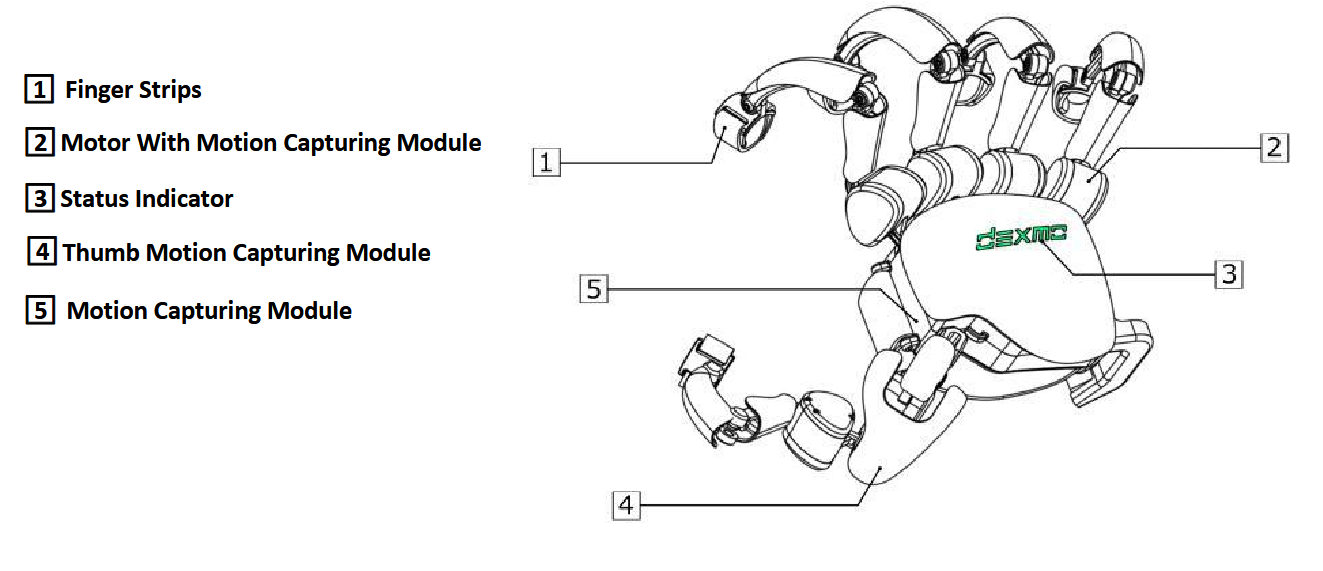
\includegraphics[width=0.8\linewidth]{chapters/exoskeleton/images/background/dexmo_glove.png}
  \caption{Design of Dexmo Glove}
  \label{fig:dexmo_glove_design}
\end{figure}

\bigskip \noindent
The Sensaglove Nova 2 uses a different approach for the force feedback. It utilizes magnetic friction brakes to transfer the force to the fingertips via mechanical wires. Each brake is capable of delivering up to 20 newtons of force, allowing for stronger haptic interactions. In addition to the force feedback, the glove integrates vibrotactile feedback to the fingertips using voice coil actuators. A hybrid approach is used for the local position tracking. The hybrid approach combines sensor-based finger tracking with computer vision hand tracking algorithms in order achieve a more accurate finger tracking with more degrees of freedom.

\bigskip \noindent
DextrES \cite{10.1145/3242587.3242657} research paper proposes a more innovative yet experimental approach. They rely on flexible metal strips to generate an electrically-controlled friction force. Such design is much more compact and light as it does not rely on motors. The haptic glove that weighs only 8g is capable of generating up to 20N of holding force for each finger. Despite being lightweight, flexible and providing strong feedback, this approach has a drawback: due to the principal of breaking, the glove can only resist and stop the movement exerted by the hand, but the virtual objects can not push against the virtual hand in order to pull your physical fingers backwards.

\begin{figure}[!h!t]
  \centering
  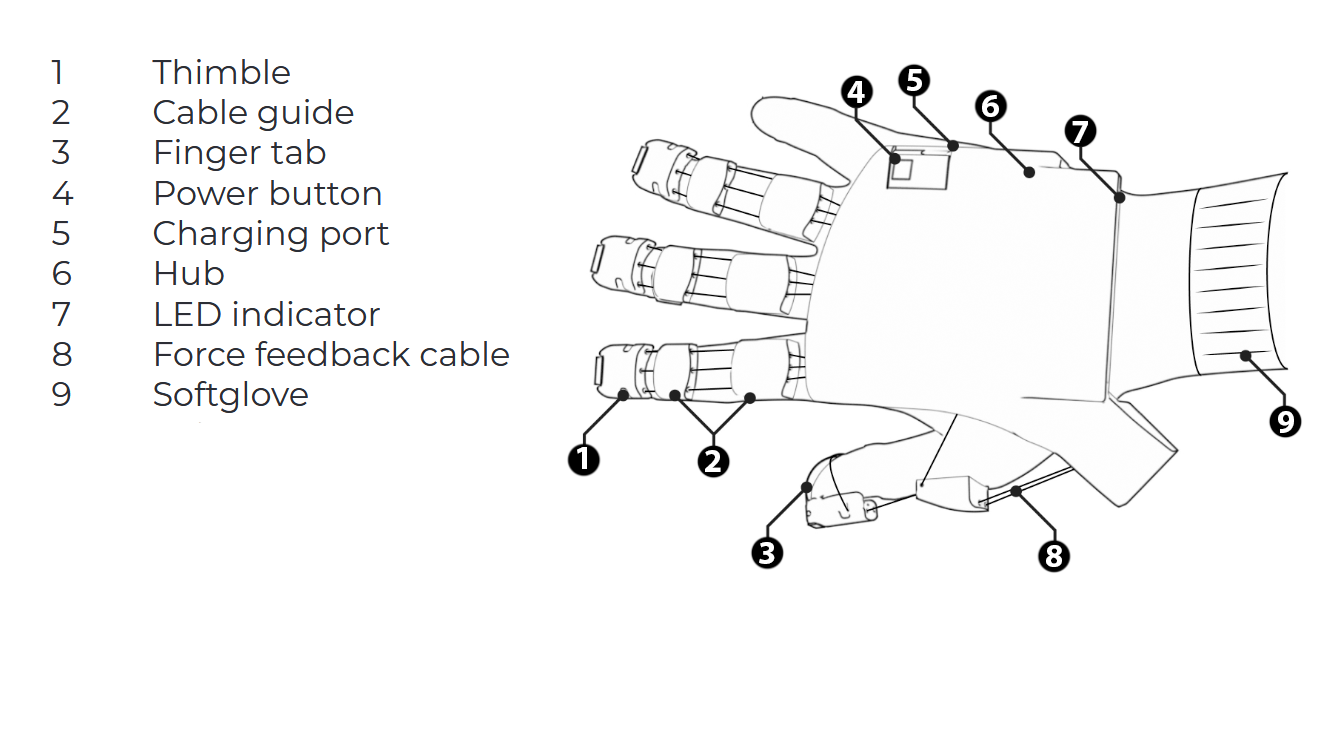
\includegraphics[width=0.8\linewidth]{chapters/exoskeleton/images/background/sensaglove.png}
  \caption{Design of Sensaglove Nova 2}
  \label{fig:sensaglove_design}
\end{figure}

\begin{figure}[!h!t]
  \centering
  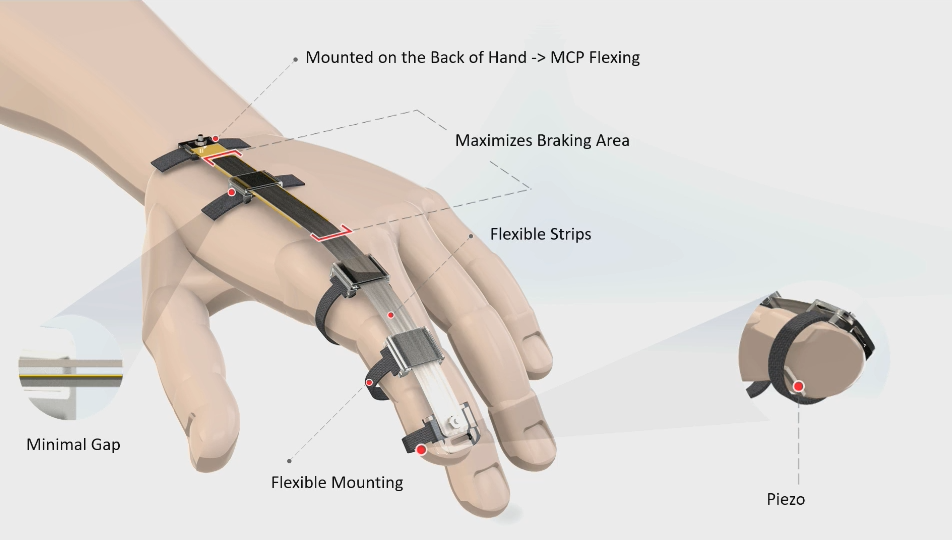
\includegraphics[width=0.8\linewidth]{chapters/exoskeleton/images/background/flexible_strips.png}
  \caption{Design of DextrES}
  \label{fig:dextrES_design}
\end{figure}

\bigskip \noindent
A distinct approach to data collection for the purpose of robot arm learning from demonstration has been proposed \cite{dai2023gripper}. The system has a gripper like form factor making the data collection intuitive. The glove uses displacement and inertial measurement unit sensors in order to capture position, orientation and gripper opening displacement information. However, unlike previously mentioned gloves, this exoskeleton provides no force feedback, its primary function is to interact with real objects rather than simulated ones. This research paper was included in this section for interesting gripper like form factor. The exoskeleton does not need to be a glove if the goal of interaction with the simulated virtual environment is to teach robots to perform tasks. 

\bigskip \noindent
Interesting approaches has been proposed for variable stiffness control using the principle of jamming. This principle relies on changing the mechanical properties of materials by altering their internal friction or structure. One such implementation is HJ-Haptic \cite{HJHaptic}, it uses this principle to provide stiffness feedback in bilateral teleoperation of robotic gripper. The device consists of flexible, honeycomb-structured layers that, when compressed through vacuum-induced suction, press together, increasing their internal friction, thereby altering the perceived stiffness. The stiffness increases linearly with the increase in pressure, allowing easy control of force feedback. A related approach has been proposed in the development of a lightweight AR glove \cite{gloveJamming}. It uses 3d printed fibers in order to achieve the layer-jamming technique for force feedback. This method ensures minimal weight and flexible finger movement, making it a promising candidate for wearable haptic interfaces.

\bigskip \noindent
Lastly, many exoskeleton researchers opt to use series elastic actuators (SEAs). This approach allows the motor to be placed outside the exoskeleton, reducing the weight and worry of needing to fit all of the components compactly on the hand. SEAs transmit the motor torque through Bowden cables. Between the motor and the load a spring is placed, to introduce compliance and enhance safety. The transmitted force is often calculated by measuring the deflection of the springs and applying a Hooke's Law, allowing for position and torque control \cite{MARCONI201969}, \cite{Refour2019}.

\bigskip \noindent
These developments in haptic exoskeletons, gloves and various prototypes exploring different mechanisms for enhancing virtual touch experiences shows that the field is evolving rapidly. While many of these technologies remain in the experimental or enterprise-focused stages, continued research and refinement is likely to bring them closer to widespread consumer adoption.